% NOTE:
% 1. Speak about electrochemical systems, their setup with the
% electrochemical cell. Mention the setup of a redox reaction.
% 2. Move into voltammetry where we change the applied potential of
% the working electrode and measure the current that is induced in
% the electrochemical cell. And then move onto mention cyclic
% voltammetry as a particular method that is popular to understand
% chemical and thermodynamical properties of the species in solution.
% 3. Elecrode kinetics as the model of how we translate the applied
% potential into the change in concentration of the species. Fast. ie
% reversible reaction approximated by the Nernst equation. But in the
% case of slower, finite, electrode kinetics we have the butler voltmer
% equation at the surface of the electrode surface.
% 4. Diffusion of the species in solution and how that brings new
% molecules to the surface and transports reduces species away from
% the surface. Mention Fick's second law that predicts how the
% diffusion causes the concentration field to change with time.

\chapter{Electrochemical Systems}

A typical electrochemical experiment uses an electrochemical cell to drive
reduction and oxidation (redox) reactions at the surface of a working
electrode. The cell consists of at least two electrodes immersed in an
electrolyte solution: the \emph{working electrode}, at whose surface the
reaction of interest takes place, and a \emph{counter electrode}, which
completes the circuit. A third \emph{reference electrode} is commonly
included to provide a stable, known potential against which the potential
of the working electrode is measured and controlled. A device called a
\emph{potentiostat} maintains the desired potential difference between the
working and reference electrodes whilst measuring the current that flows
between the working and counter electrodes.

A one-electron redox reaction can be written as:
\begin{equation}\label{eq:redox}
  \mathrm{A} + \mathrm{e}^{-} \rightleftharpoons \mathrm{B},
\end{equation}
where species $\mathrm{A}$ is reduced -- that is, it gains one electron --
to form species $\mathrm{B}$. The reverse process, in which $\mathrm{B}$
loses an electron to regenerate $\mathrm{A}$, is the corresponding
oxidation.

\section{Voltammetry}

Voltammetry is the class of electroanalytical techniques in which the
potential applied to the working electrode is varied in a prescribed
manner and the resulting current is recorded. Because the current is
directly related to the rate of the electrochemical reaction at the
electrode surface, the current--potential curve -- called a
\emph{voltammogram} -- encodes information about the thermodynamics and
kinetics of the redox process as well as the transport of chemical species
in solution.

In a cyclic voltammetry (CV) experiment the applied potential is swept
linearly with time from some starting potential $E_i$, at which the
species $\mathrm{A}$ is stable and no significant reaction occurs, to a
vertex potential $E_v$, at which electron transfer occurs rapidly to form
species $\mathrm{B}$. The potential is then swept back to $E_i$, causing
electron transfer in the opposite direction and the reformation of
$\mathrm{A}$. This triangular waveform is illustrated in the left panel of
\autoref{fig:potential_voltammagram}.

Throughout this process the current $I$ is recorded. Plotting the current
against the applied potential gives the voltammogram shown in the right
panel of \autoref{fig:potential_voltammagram}. The forward sweep produces
a reduction (cathodic) peak as the potential moves through the range at
which $\mathrm{A}$ is converted to $\mathrm{B}$; the return sweep produces
an oxidation (anodic) peak as $\mathrm{B}$ is reconverted to $\mathrm{A}$.
The peak shape arises from competition between the electrode kinetics,
which accelerate as the driving potential increases, and the depletion of
$\mathrm{A}$ near the electrode surface caused by the ongoing reaction.

\begin{figure}
  \begin{center}
    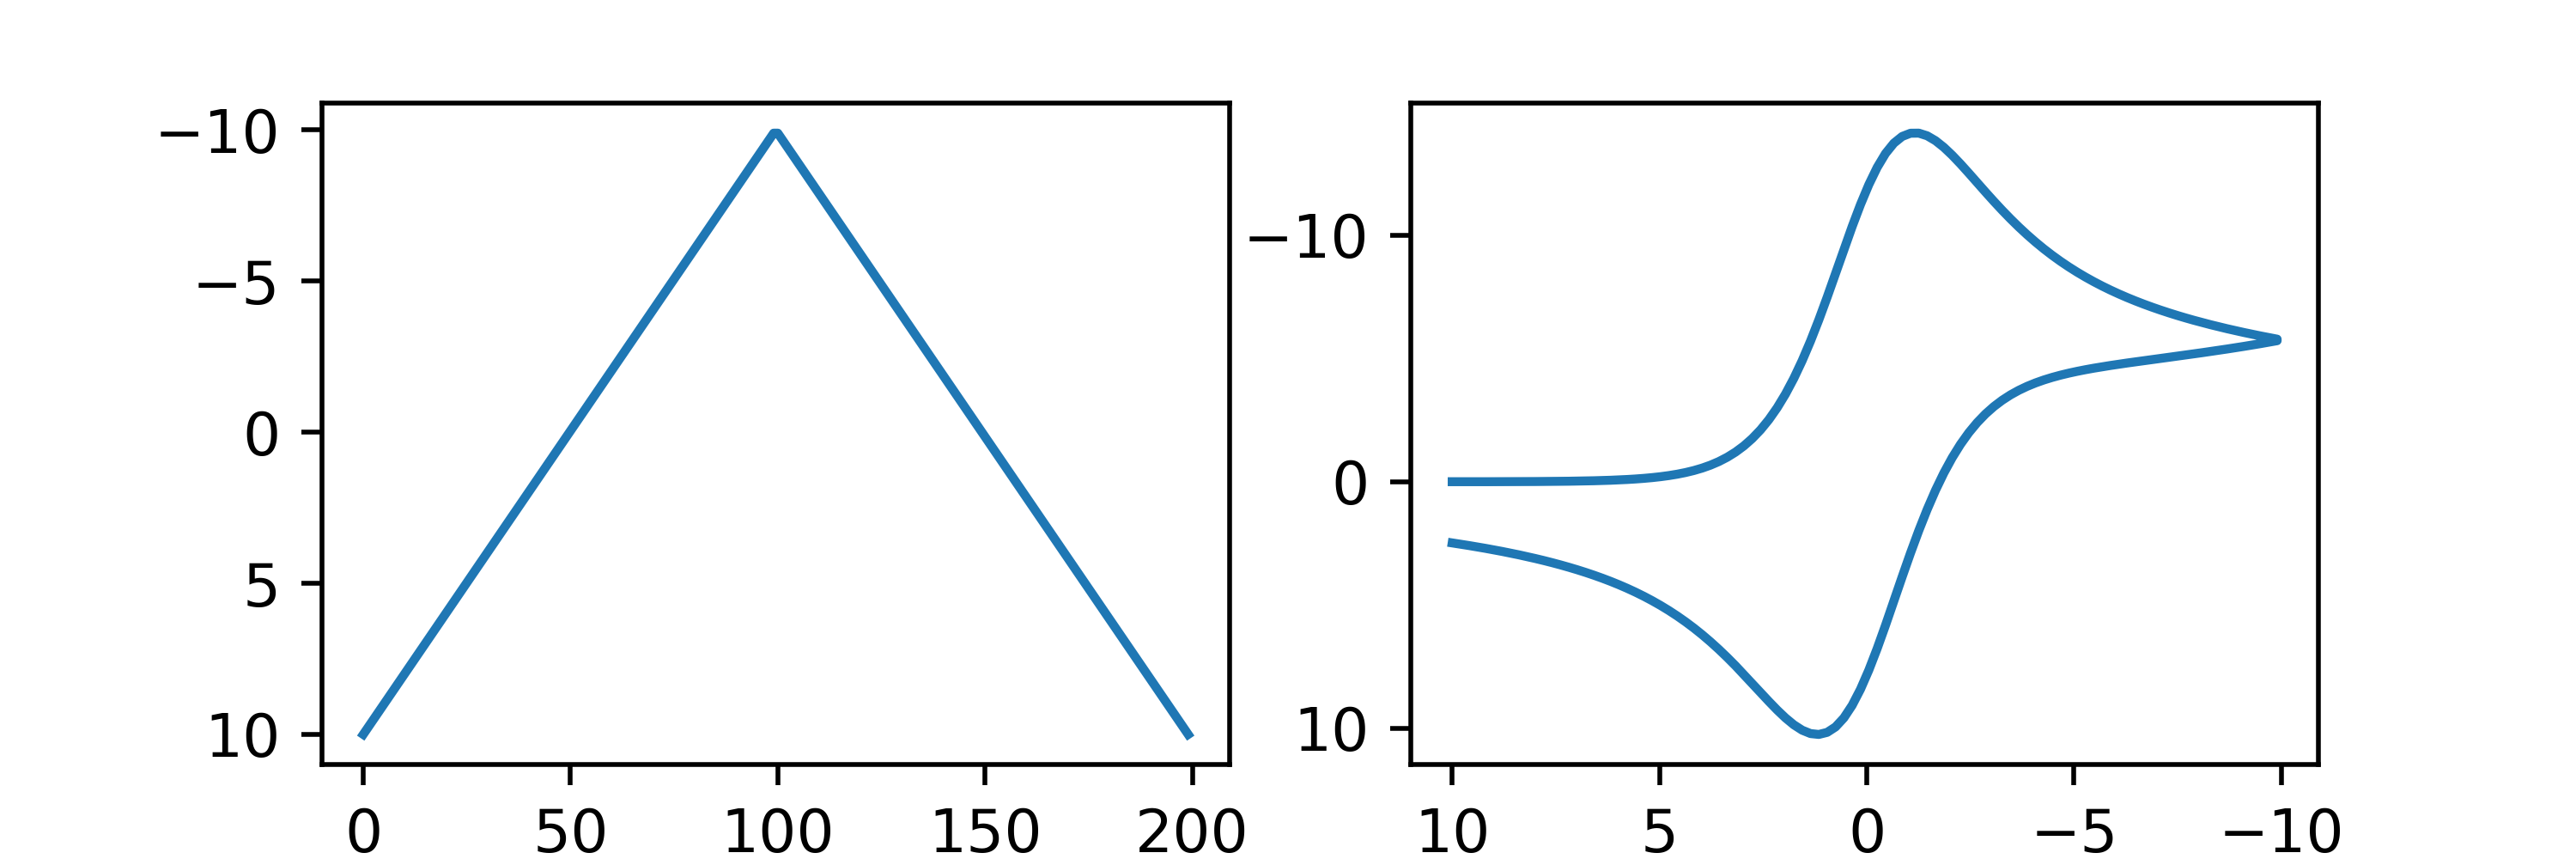
\includegraphics[width=0.95\textwidth]{figures/figure_1_voltammagram.png}
  \end{center}
  \caption[Applied potential and voltammogram example]{Left: the triangular
    potential waveform applied in a cyclic voltammetry experiment. Right:
    the resulting voltammogram showing cathodic (reduction) and anodic
  (oxidation) current peaks.}
  \label{fig:potential_voltammagram}
\end{figure}

This technique is particularly useful because the position, shape, and
relative heights of the peaks provide a signature of the
electrochemical process. The potential at which each peak occurs is related
to the standard reduction potential $E^{\circ}$, and the separation between
the cathodic and anodic peaks carries information about the electrode
kinetics, as discussed in \autoref{sec:electrode_kinetics}.

The \emph{scan rate} $\nu$ $(\mathrm{V\,s^{-1}})$ is the constant rate at
which the potential is swept, defined as
\begin{equation}
  \nu = \frac{dE}{dt}.
\end{equation}
The scan rate is an important experimental parameter: faster scans probe
shorter timescales and can resolve kinetic processes that would otherwise
reach equilibrium on a slower scan, whilst slower scans allow more time for
diffusion and can reveal coupled chemical reactions.

\section{Electrode Kinetics}\label{sec:electrode_kinetics}

In order to model the reaction~\eqref{eq:redox} in a voltammetry
experiment we require a description of how the applied potential drives
the interconversion of $\mathrm{A}$ and $\mathrm{B}$ at the electrode
surface. The electrode reaction rate is commonly expressed through the
\emph{flux} $J$ $(\mathrm{mol\,m^{-2}\,s^{-1}})$ of material consumed or
produced at the surface.

\subsection{The Nernst Equation: Reversible Kinetics}

When the rate of electron transfer is very fast relative to the timescale
of the experiment, the concentrations of $\mathrm{A}$ and $\mathrm{B}$ at
the electrode surface are in thermodynamic equilibrium with the applied
potential at every instant. In this \emph{reversible} (or
\emph{Nernstian}) limit, the surface concentrations $c_{\mathrm{A}}(0,t)$
and $c_{\mathrm{B}}(0,t)$ are related to the applied potential $E(t)$ by
the Nernst equation,
\begin{equation}\label{eq:nernst}
  E(t) = E^{\circ} + \frac{RT}{F}
  \ln\frac{c_{\mathrm{A}}(0,t)}{c_{\mathrm{B}}(0,t)},
\end{equation}
where $R$ is the universal gas constant, $T$ is the absolute temperature,
and $F$ is Faraday's constant. Equation~\eqref{eq:nernst} serves as a
boundary condition at the electrode surface; combined with the diffusion
equation introduced in \autoref{sec:diffusion}, it fully determines the
concentration fields and hence the current in the reversible limit.

\subsection{The Butler--Volmer Equation: Finite Electrode Kinetics}

When the electron-transfer rate is finite, the surface concentrations
depart from the Nernstian equilibrium values, and the reaction rate must
be modelled explicitly. The standard model for electrode kinetics is the
\emph{Butler--Volmer} equation \cite{dickinson2020butler}, which
gives the flux at the electrode
surface as
\begin{equation}\label{eq:butler_volmer}
  J = k_{0}\!\left[c_{\mathrm{A}}(0,t)\,
    \exp\!\left(-\frac{\alpha F}{RT}\eta(t)\right)
    - c_{\mathrm{B}}(0,t)\,
  \exp\!\left(\frac{(1-\alpha) F}{RT}\eta(t)\right)\right],
\end{equation}
where $k_{0}$ $(\mathrm{m\,s^{-1}})$ is the standard rate constant,
$\alpha \in (0,1)$ is the transfer coefficient (often taken to be $0.5$
for a symmetric energy barrier), and
\begin{equation}
  \eta(t) = E(t) - E^{\circ}
\end{equation}
is the \emph{overpotential}, measuring the deviation of the applied
potential from the equilibrium value. The two exponential terms in
\eqref{eq:butler_volmer} represent the reduction and oxidation
contributions respectively: a negative overpotential ($E < E^{\circ}$)
drives reduction, whilst a positive overpotential drives oxidation.

The Butler--Volmer equation interpolates naturally between two limits.
When $k_{0}$ is large, the exponential terms force the surface
concentrations towards the Nernstian equilibrium values~\eqref{eq:nernst},
recovering reversible behaviour. When $k_{0}$ is small, the reaction is
kinetically limited and the flux is directly proportional to $k_{0}$,
giving \emph{irreversible} behaviour. The current measured in the external
circuit is related to the flux by
\begin{equation}
  I(t) = F A\, J(t),
\end{equation}
where $A$ $(\mathrm{m}^2)$ is the electrode area.

\section{Diffusion}\label{sec:diffusion}

The electrode reaction consumes $\mathrm{A}$ and produces $\mathrm{B}$ at
the surface. Fresh $\mathrm{A}$ must therefore be transported from the
bulk of the solution to the electrode, and $\mathrm{B}$ must be
transported away. In quiescent (unstirred) solutions, the dominant
transport mechanism is \emph{diffusion}: the net movement of molecules
down concentration gradients driven by random thermal motion.

We model each species by a concentration field $c(x,t)$, where $x$
denotes the distance from the electrode surface and $t$ denotes time.
For a planar electrode, the evolution of the concentration is governed by
\emph{Fick's second law} \cite{crank1979mathematics},
\begin{equation}\label{eq:ficks_second}
  \frac{\partial c}{\partial t} = D\frac{\partial^{2} c}{\partial x^{2}},
\end{equation}
where $D$ $(\mathrm{m}^2\,\mathrm{s}^{-1})$ is the diffusion coefficient
of the species. Equation~\eqref{eq:ficks_second} is a linear
parabolic partial differential equation.

For the couple $\mathrm{A}/\mathrm{B}$ we therefore have a system of two
diffusion equations,

\begin{align}
  \frac{\partial c_{\mathrm{A}}}{\partial t}
  &= D_{\mathrm{A}}\frac{\partial^{2} c_{\mathrm{A}}}{\partial x^{2}},
  \label{eq:diffusion_A}\\
  \frac{\partial c_{\mathrm{B}}}{\partial t}
  &= D_{\mathrm{B}}\frac{\partial^{2} c_{\mathrm{B}}}{\partial x^{2}},
  \label{eq:diffusion_B}
\end{align}

where $D_{\mathrm{A}}$ and $D_{\mathrm{B}}$ are the respective diffusion
coefficients. These equations hold on the semi-infinite domain $x > 0$,
representing the bulk solution, and are supplemented by initial conditions
and boundary conditions. Initially the solution is homogeneous:
\begin{equation}
  c_{\mathrm{A}}(x,0) = c_{\mathrm{A}}^{\ast}, \qquad
  c_{\mathrm{B}}(x,0) = 0,
\end{equation}
where $c_{\mathrm{A}}^{\ast}$ is the bulk concentration of $\mathrm{A}$.
Far from the electrode the concentrations recover their bulk values,
\begin{equation}
  c_{\mathrm{A}}(x,t) \to c_{\mathrm{A}}^{\ast}, \qquad
  c_{\mathrm{B}}(x,t) \to 0 \qquad \text{as } x \to \infty,
\end{equation}
whilst at the electrode surface ($x = 0$) the diffusive fluxes are
coupled to the electrode reaction through flux-conservation conditions.
Conservation of matter at the surface requires
\begin{equation}\label{eq:flux_conservation}
  D_{\mathrm{A}}\frac{\partial c_{\mathrm{A}}}{\partial x}\bigg|_{x=0}
  = -D_{\mathrm{B}}\frac{\partial c_{\mathrm{B}}}{\partial x}\bigg|_{x=0}
  = J(t),
\end{equation}
where $J(t)$ is the reaction flux given by the Butler--Volmer
equation~\eqref{eq:butler_volmer} (or, in the reversible limit, determined
  implicitly by the Nernst equation~\eqref{eq:nernst} together with the
constraint~\eqref{eq:flux_conservation}).

The complete mathematical description -- comprising the two diffusion
equations~\eqref{eq:diffusion_A} -- \eqref{eq:diffusion_B}, the initial and
far-field conditions, and the surface boundary conditions -- constitutes a
well-posed initial-boundary value problem whose solution gives the
concentration fields and, via~\eqref{eq:flux_conservation}, the current
$I(t)$ as a function of time during a cyclic voltammetry experiment. The
remainder of this thesis is concerned with the analysis and numerical
solution of this problem.

\subsection{Dimensionless Coordinates}

There are many non-dimensionalisations that can be performed on the
described problem. We follow the transformations similar to those done
in \cite{compton2014understanding}

\begin{tabular}{ll}
  \hline Parameter & Normalisation \\
  \hline concentration & $C_j=c_j / c_{\mathrm{A}}^*$ \\
  diffusion coefficient & $d_j=D_j / D_{\mathrm{A}}$ \\
  spatial coordinate & $X=x / \epsilon$ \\
  time & $T=D_{\mathrm{A}} t / \epsilon^2$ \\
  potential & $\theta=(\mathrm{F} / \mathcal{R}
  \mathcal{T})\left(E-E_{\mathrm{f}}^0\right)$ \\
  scan rate & $\sigma=\left(\epsilon^2 /
  D_{\mathrm{A}}\right)(\mathrm{F} / \mathcal{R} \mathcal{T}) \nu$ \\
  current & $J=I /\left(\pi \epsilon \mathrm{F} D_{\mathrm{A}}
  c_{\mathrm{A}}^*\right)$ \\
  \hline
\end{tabular}
